%!TEX program = xelatex
%!TEX option = --output-driver="xdvipdfmx -V7"
\documentclass[xcolor=dvipsnames,hyperref={CJKbookmarks=true},aspectratio=169]{beamer}
% \usetheme{CambridgeUS}
% \usecolortheme{dolphin}
% \usefonttheme{professionalfonts}
% \setbeamertemplate{bibliography item}{}
\usepackage{appendixnumberbeamer}
\usepackage{tcolorbox}
\usepackage{xcolor}
\definecolor{whitesmoke}{rgb}{0.96, 0.96, 0.96}
\setbeamerfont{page number in head/foot}{size=\large}
\setbeamertemplate{footline}[frame number]
\mode<presentation>
\usetheme{Berkeley}
\renewcommand\appendixname{Appendix}

\setbeamercolor{postit}{bg=MidnightBlue}
\usecolortheme[named=MidnightBlue]{structure}
\useinnertheme{rounded}  
\usefonttheme[onlymath]{serif}

\beamertemplatenavigationsymbolsempty

\usepackage{lmodern}
\graphicspath{{figure/}}

\usepackage{amsmath,amssymb,esint} 
\allowdisplaybreaks[0]
\usepackage{siunitx}
\usepackage{graphicx} 
\usepackage{array} 
\usepackage{multirow} 
\usepackage{braket}

\usepackage{tikz}
\usetikzlibrary{quotes,angles}
\usetikzlibrary{3d,calc}
\usetikzlibrary{shapes.geometric}
\usetikzlibrary{arrows,positioning}

\newcommand{\dif}{\,\mathrm d}
\newcommand\mi{\mathrm{i}}
\newcommand\e{\mathrm{e}}
\newcommand{\rf}{\text{rf}}
\newcommand{\thm}{\text{th}}
\DeclareMathOperator{\Hc}{H.c.}
\DeclareMathOperator{\Tr}{Tr}

% \usepackage[style=authoryear-comp,sorting=none]{biblatex}
% \bibliography{photonnumber}
\bibliographystyle{plain}
\setbeamertemplate{bibliography item}[triangle]

\title[Nature 445, 515-518]{Resolving photon number states in a superconducting circuit}
\author[Ming, Elena]{Ming Lyu, Elena de la Hoz Lopez-Collado}
\institute[Princeton]{Final projects for ELE456 at Princeton}
\date{May 11, 2017}
\logo{
\includegraphics[width=1cm]{Princetonshield}}
\begin{document}
\begin{frame}
\titlepage
\end{frame}
\begin{frame}
    \tableofcontents
\end{frame}

\section{Introduction} 
% \begin{frame}[t]\frametitle{The paper}
    
% This is for paper \cite{schuster2007resolving} % To show bib

% \end{frame}

\begin{frame}
\frametitle{Outline}
\begin{itemize}
\item Resolve photon number states in a circuit QED
\vspace{0.3cm}
\item System: superconducting qubit +  microwave transmission line
\vspace{0.3cm}
\item Strong dispersive regime
\vspace{0.3cm}
\item Spectroscopic measurements: \\
Qubit's spectral lines different for each photon number state
\end{itemize}
\end{frame}

\section{Experiment implementdeation}

\subsection{Cavity QED}
% Say we work with qubits!
\begin{frame}
\frametitle{The system: circuit QED + cavity QED}
\begin{figure}
\centering
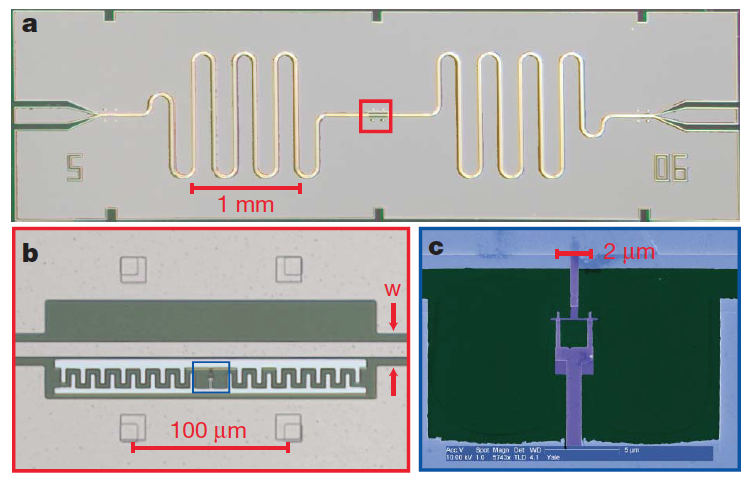
\includegraphics[width=0.7\linewidth]{Circuit.png}
\end{figure}
\tiny{\textcolor{gray}{Image from Schuster, D. I., et al. "Resolving photon number states in a superconducting circuit." Nature 445.7127 (2007): 515-518.\cite{schuster2007resolving}}}
\end{frame}

\begin{frame}
\frametitle{The system: simplified}
% \begin{itemize}
% \item Cavity QED (cQED) $\rightarrow$ interaction electromagnetic field modes with superconducting qubit
% \end{itemize}
\begin{figure}
\centering
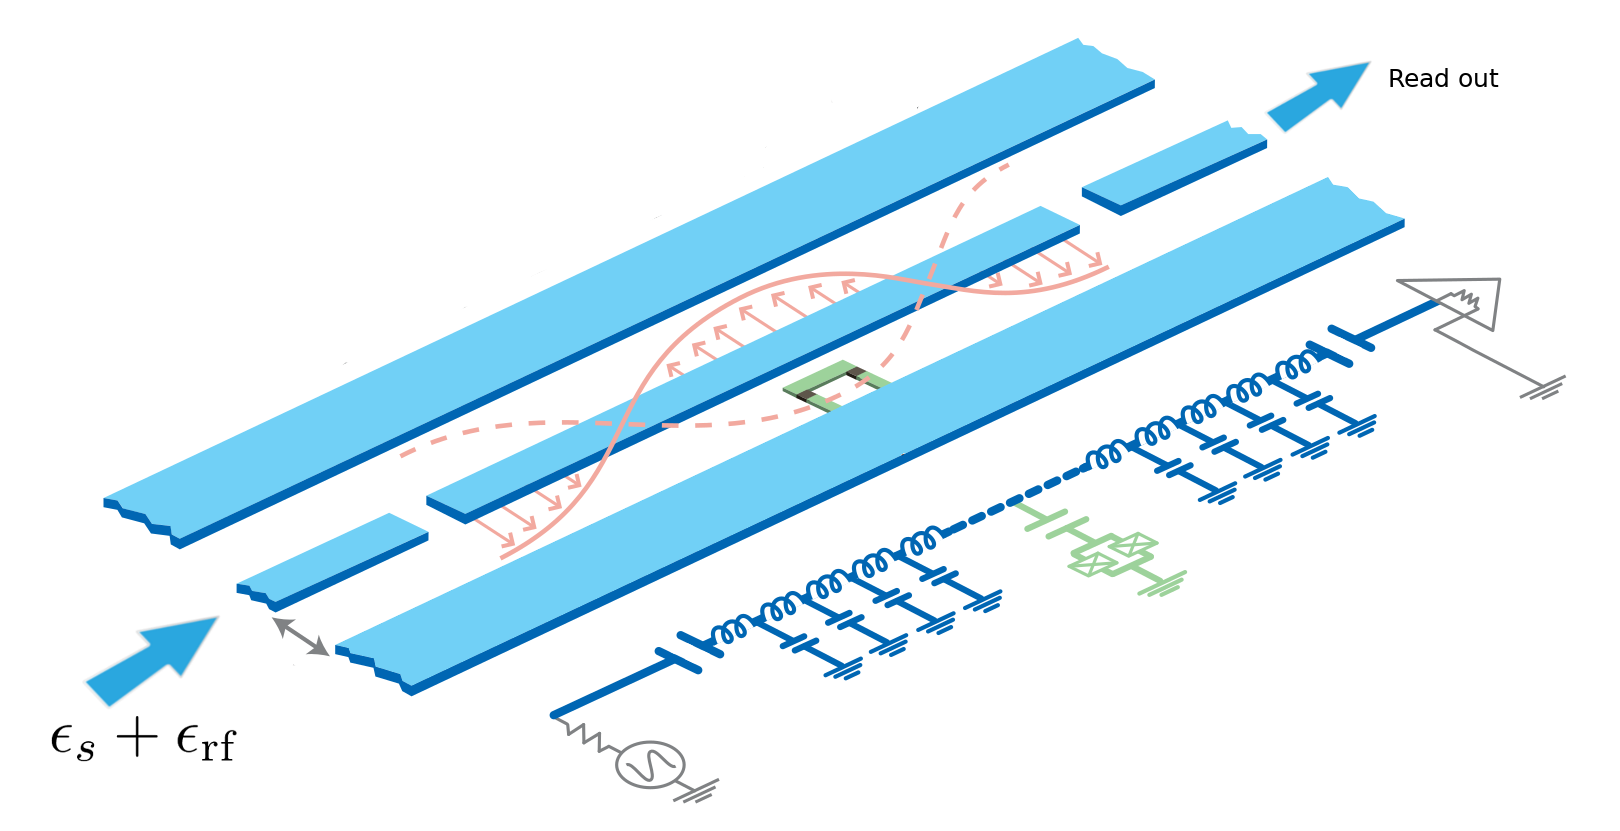
\includegraphics[width=0.85\linewidth]{cavity.png}
\end{figure}
\tiny{\textcolor{gray}{Image from Blais, Alexandre, et al. "Cavity quantum electrodynamics for superconducting electrical circuits: An architecture for quantum computation." Physical Review A 69.6 (2004): 062320.\cite{blais2004cavity}}}
\end{frame}

\section{The model}
\begin{frame}
\frametitle{Cavity QED: the Hamiltonian}
\begin{block}{Hamiltonian}
$$H =  \omega_r \left(a^{\dagger} a+ \dfrac{1}{2} \right) +  \omega_a \dfrac{\sigma^{z}}{2}+  g \left(a^{\dagger}\sigma^{-}+a\sigma^{+}\right)$$
\end{block}
\vspace{0.5cm}
\begin{itemize}
\item $\omega_r$: cavity resonance frequency
\vspace{0.3cm}
\item $\omega_a$: qubit transition frequency
\vspace{0.3cm}
\item $g$: strength qubit-photon coupling
\vspace{0.3cm}
\item $\Delta = \omega_r - \omega_a$: detuning between qubit and cavity
\end{itemize}
\end{frame}


\begin{frame}
\frametitle{Strong Dispersive Regime}
\begin{figure}
\centering
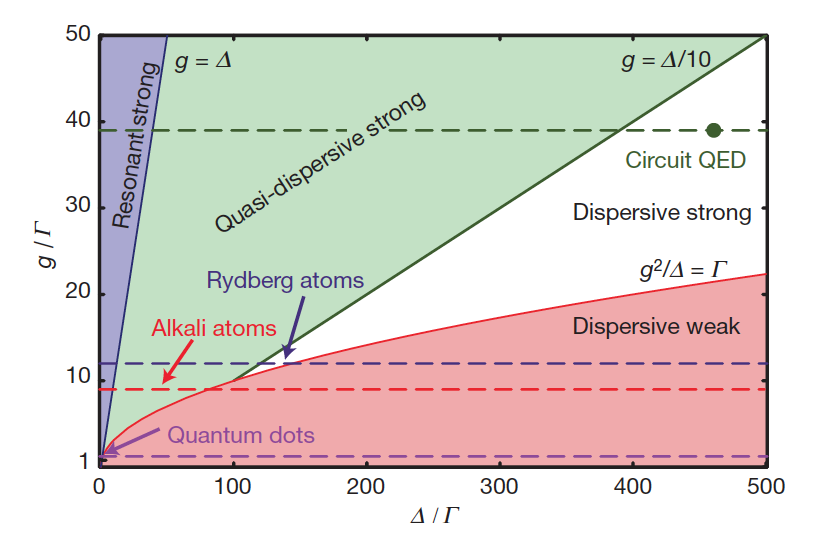
\includegraphics[width=0.7\textwidth]{Regime}
\end{figure}

\tiny{\textcolor{gray}{Image from Schuster, D. I., et al. "Resolving photon number states in a superconducting circuit." Nature 445.7127 (2007): 515-518.\cite{schuster2007resolving}}}
\end{frame}

\begin{frame}
\frametitle{Strong dispersive Regime: Diagonalization}
\begin{itemize}
\item Transformation: 
$$U=\exp{\left(\dfrac{g}{\Delta}\left(a\sigma^{+}-a^{\dagger}\sigma^{-} \right)\right)}$$
\item Hamiltonian to first order in $\dfrac{g}{\Delta}$ (dispersive regime):
\begin{eqnarray*}
H_0 &=& U\,H\,U^{\dagger}\\
&\simeq &  \omega_r \left(a^{\dagger} a+ \dfrac{1}{2} \right) +  \omega_a \dfrac{\sigma^{z}}{2}+ \chi \left(a^{\dagger}a+\dfrac{1}{2} \right)\dfrac{\sigma^{z}}{2}
\end{eqnarray*}
where $\chi = g/\Delta ^2$
\end{itemize}
\end{frame}

\subsection{Driving terms}
\begin{frame}\frametitle{Spectrum of the system}
\begin{figure}
\centering
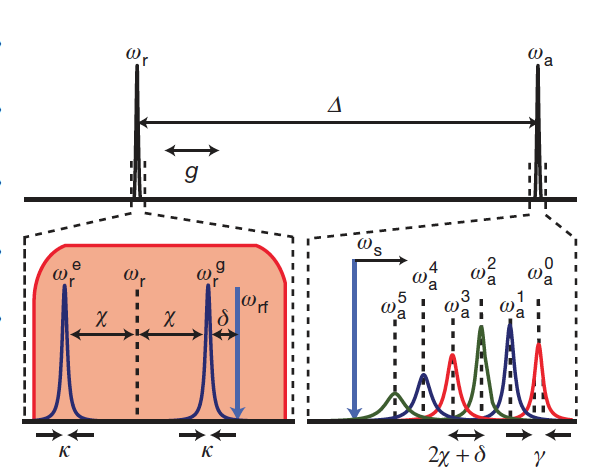
\includegraphics[width=0.55\linewidth]{TransitionLines}
\end{figure}
\tiny{\textcolor{gray}{Image from Schuster, D. I., et al. "Resolving photon number states in a superconducting circuit." Nature 445.7127 (2007): 515-518.\cite{schuster2007resolving}}}
\end{frame}

\begin{frame}
\frametitle{Driving terms}
\begin{itemize}
\item To conduct a measurement we first drive the cavity:
    $$
      H_{\rf} = \epsilon_{\rf}\left(a^{\dagger}\e^{-\mi\omega_{\rf}t}
      +a\e^{\mi\omega_{\rf}t} \right)
    $$
with $\omega_{\rf}$ near $\omega_r$
\item The frequency shift of the qubit measured with a sweeping signal
    $$
      H_{s} = \epsilon_{s}\left(a^{\dagger}\e^{-\mi\omega_{s}t}
      +a\e^{\mi\omega_{s}t} \right)
    $$
with $\omega_{s}$ near $\omega_a$
\item Note that relative strength of $\epsilon_s$ is not mentioned. We treat it 
as a perturbation. 
\end{itemize}
\end{frame}

\begin{frame}
\frametitle{Rotating frame and Rotating wave approximation}
\begin{itemize}
\item Applying the transformation
$$U=\exp\left[\dfrac{g}{\Delta}\left(a\sigma^{+}-a^{\dagger}\sigma^{-} \right)\right]$$
\item And moving to the rotating frame:
$$U_I=\exp\left[\mi t\left(
\omega_{\rf}a^{\dagger}a +\omega_s\sigma^{z}/2 \right)\right]$$
\end{itemize}
Under rotating frame, $H_{\rf}$ and $H_{s}$ are (with RWA):
\begin{align*}
	&H_{\rf} = \epsilon_{\rf}\left(a^{\dagger}+a\right) \\
	&H_{s} = \left(\frac{g}{\Delta}\right)\epsilon_{s}\left(\sigma^{+}+\sigma^{-} \right)
\end{align*}
\end{frame}

\begin{frame}
\frametitle{Final Hamiltonian and collapse operators}
\begin{itemize}
	\item Full Hamiltonian: 
\begin{align*}
H =& \omega_r \left(a^{\dagger} a+ \dfrac{1}{2} \right) +  \omega_a \dfrac{\sigma^{z}}{2}+ \chi \left(a^{\dagger}a+\dfrac{1}{2} \right)\dfrac{\sigma^{z}}{2}\\
& - \left( \omega_{\rf}a^{\dagger}a +\omega_s \dfrac{\sigma^{z}}{2} \right) + \epsilon_{\rf}\left(a^{\dagger}+a\right) 
+  \epsilon_{s}\dfrac{g}{\Delta}\left(\sigma^{+}+\sigma^{-} \right)
\end{align*}
	\item Collapse operator: 
	\begin{itemize}
		\item  Collapse operators cavity: 
		$\sqrt{\kappa \left(1+n_{\thm} \right)}a$, 
		$\sqrt{\kappa n_{\thm} }a^{\dagger}$
		\item Collapse operator qubit:  
		$\sqrt{\gamma}\sigma^{-}$
		\item Dephasing: 
		$\sqrt{\gamma_{\phi}}\sigma^{z}$
	\end{itemize}
\end{itemize}
\end{frame}

% \subsection{Diagonal under strong dispersive limit}
% \subsection{Rotating wave approximation}
% \subsection{Dissipation: the collapse operators}
\subsection{Measurement}
\begin{frame}[t]\frametitle{Measurement}
	\begin{itemize}
		\item In the experiment, the transmitted amplitude at frequency $\omega_{\rf}$ is the main observable under steady state. 
	\begin{block}{Steady state}
	$$
	\dot\rho_s = 0 = -\mi[H, \rho_{s}] + \sum_n \left(2C_n \rho_s C_n^\dag - 
	\{\rho_s, C_n^\dag C_n\}\right)
	$$
	\end{block}
	~

		\item What they really measure is the expectation of the 
		electrical field $E\propto\langle a + a^\dag \rangle$ \cite{schuster2007circuit} on a given frequency
	$$
	E\propto \langle a + a^\dag \rangle = \Tr [\rho_{s}(a+a^\dag)]
	$$
	\end{itemize}
\end{frame}

\section{Numerical simulation}
\subsection{Property of the cavity}
\begin{frame}[t]\frametitle{Property of the cavity: Analytical}
\begin{itemize}
	\item Without the qubit, the cavity state is equivalently a damped harmonic oscillator with driving
	$$
	 H = \delta a^\dag a + \epsilon (a + a^\dag)
	$$
	Collapse operators: $\sqrt{\kappa(n_{\thm}+1)}a$ and 
	$\sqrt{\kappa n_{\thm}}a^\dag$
	\item When it's off resonant, its steady state is not but approximately a coherent state
	\item Analytically the photon number expectation value is 
	$$
	\bar n = \frac{\epsilon^2}{\delta^2 + \kappa^2/4} + n_{\thm}
	$$
\end{itemize}
\end{frame}

\begin{frame}[t]\frametitle{Property of the cavity: Numerical}
\begin{itemize}
	\item Numerically, a truncate on Fock space is needed
	\item To check the validity of the truncate, we plot the photon distribution 
	and frequency response of the cavity. 
\end{itemize}
\begin{columns}
\begin{column}{0.5\linewidth}
	\centering
    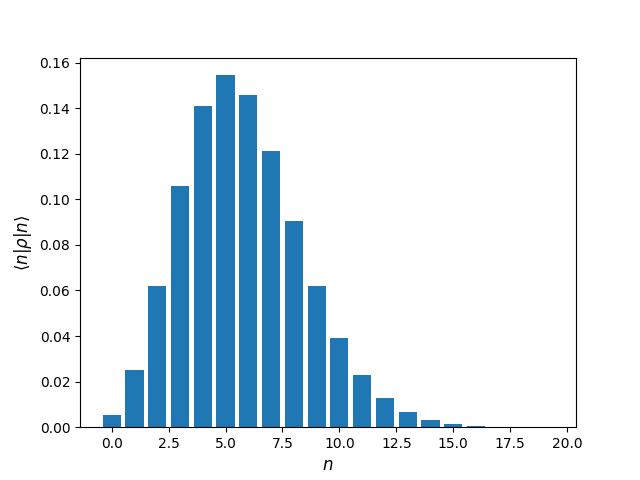
\includegraphics[width=\textwidth]{photon_number_dist.png}
\end{column}%
\begin{column}{0.5\linewidth}
	\centering
    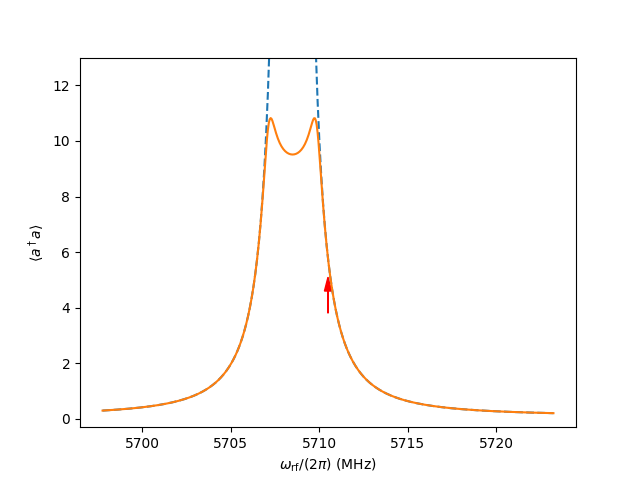
\includegraphics[width=\textwidth]{resonance.png}
\end{column}
\end{columns}
\end{frame}

\subsection{Reproduce results}
\begin{frame}[t]\frametitle{Direct spectroscopic observation of quantized cavity photon number}
\begin{columns}
\begin{column}{0.4\linewidth}
% \begin{itemize}
	For a fixed driving $\epsilon_{\rf}$, plot the reduction
	$V_0 - \langle a^\dag + a\rangle_{ss}$ v.s. $\omega_{s}$. 

~

	$\epsilon_{\rf}$ is labeled by $\bar n$ with relationship:
	\begin{equation*}
		\bar n = n_{\thm} + \frac{\epsilon_{\rf}^2}{\delta^2 + \kappa^2/4}
	\end{equation*}
% \end{itemize}
\end{column}%
\begin{column}{0.6\linewidth}
	\centering
    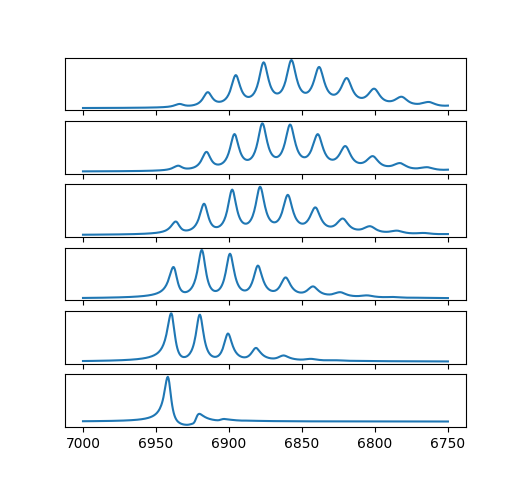
\includegraphics[width=0.9\textwidth]{sweaping.png}
\end{column}
\end{columns}
\end{frame}

\begin{frame}[t]\frametitle{Direct spectroscopic observation of quantized cavity photon number: compare}
\begin{columns}
\begin{column}{0.35\linewidth}
    \centering
    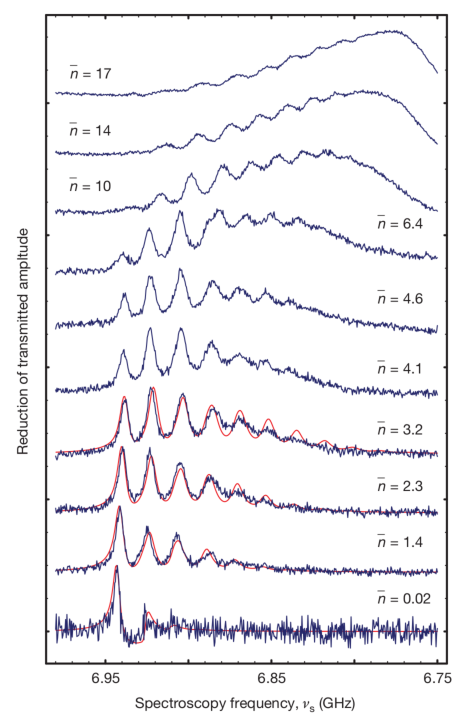
\includegraphics[width=0.7\linewidth]{sweaping_origin.pdf}
    % \caption{Original results (theory: red lines)}
\end{column}%
\begin{column}{0.65\linewidth}
	\centering
    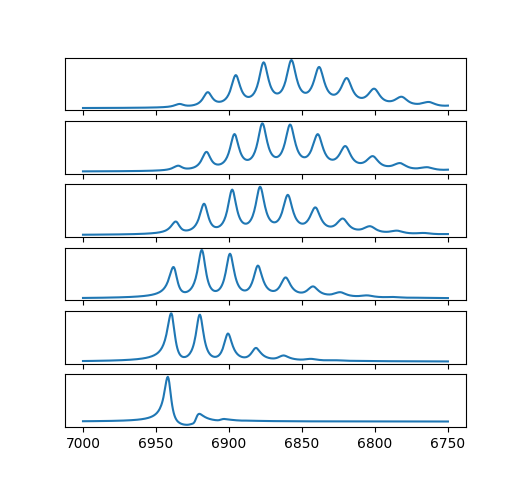
\includegraphics[width=0.7\linewidth]{sweaping.png}
\end{column}
\end{columns}
\begin{itemize}
	% \item The way $\bar n$ is defined is larger than ours. 
	\item Fits well with small $\bar n$, but other noise becomes significant 
	for larger $\bar n$
\end{itemize}
\end{frame}

\begin{frame}[t]\frametitle{Strengthen? }
\begin{center}
	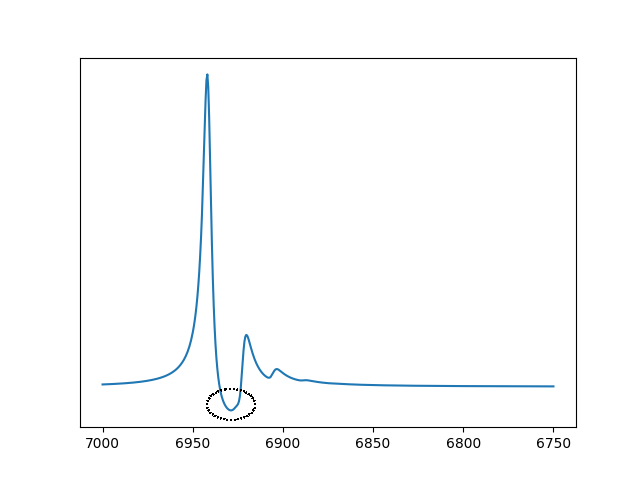
\includegraphics[width=0.55\linewidth]{figure/erf=0.1.png}
\end{center}
For small RF signal, there's a range where the transmitted amplitude is increased. 
We'll explain it later. 
\end{frame}

\begin{frame}[t]\frametitle{Thermal Drive}
\begin{itemize}
	\item Thermal Drive is equivalent to setting $n_{\thm}$ in collapse operator
	to the driving average, with small $\epsilon_{\rf}$ to show the phase 
	lock-in at the given frequency. 
\end{itemize}
	\centering
    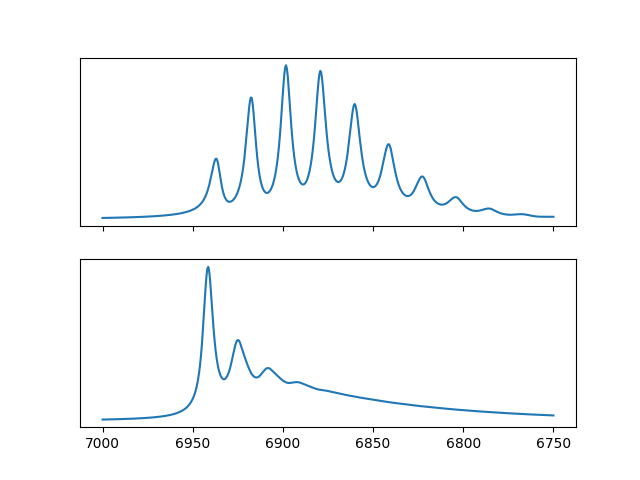
\includegraphics[width=0.55\textwidth]{thermal.png}
\end{frame}

\begin{frame}[t]\frametitle{Thermal Drive: compare}
\begin{columns}
\begin{column}{0.4\linewidth}
    \centering
    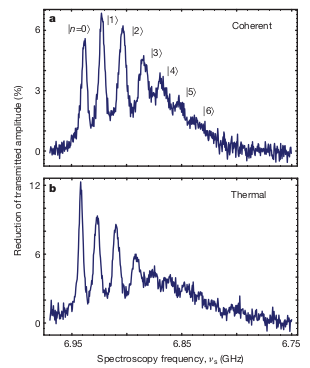
\includegraphics[width=0.8\linewidth]{thermal_origin.png}
    % \caption{Original results (theory: red lines)}
\end{column}%
\begin{column}{0.6\linewidth}
	\centering
    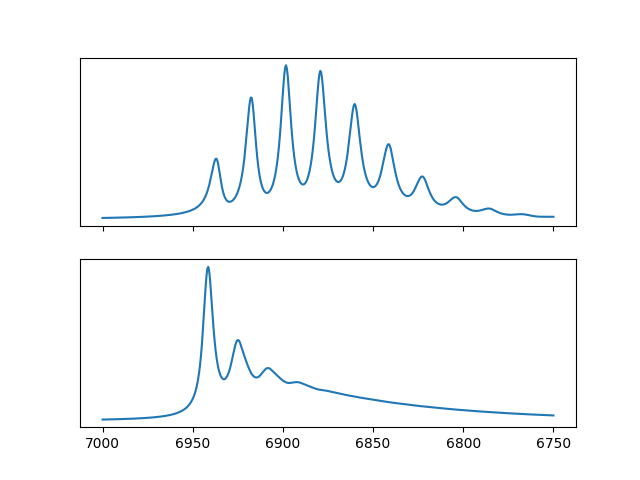
\includegraphics[width=0.9\linewidth]{thermal.png}
\end{column}
\end{columns}
\begin{itemize}
	\item Note that there's no thermal drive theory fitting. 
	Our results tracks fewer peaks, but this depends on 
	how they do the measurement, which is not mentioned in the paper. 
\end{itemize}
\end{frame}

\section{Discussion}
\begin{frame}[t]\frametitle{Discussion: The picture of what happens}
\begin{itemize}
	\item The peaks shows discreteness in the photon state in the cavity. 
	\item Exciting the qubit making the cavity off-resonance, which results in
	the reduction? \pause \textbf{\color{red} NOT TRUE} \pause
	\item Expected photon number increases at the peaks!
\begin{columns}
\begin{column}{0.5\linewidth}
    \centering
    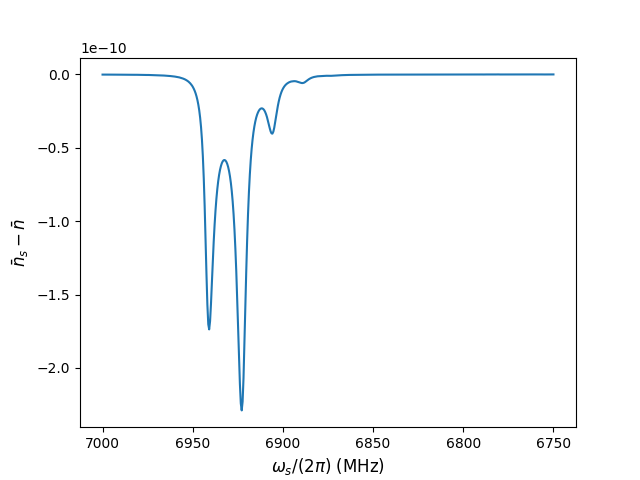
\includegraphics[width=\linewidth]{nbar_1.png}
\end{column}%
\begin{column}{0.5\linewidth}
	\centering
    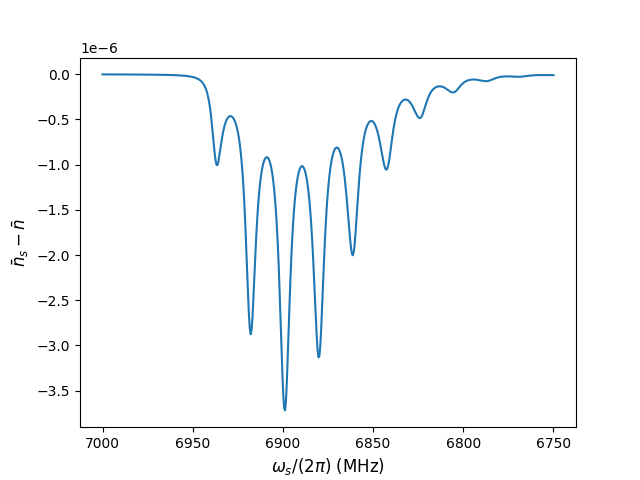
\includegraphics[width=\linewidth]{nbar_2.png}
\end{column}
\end{columns}
\end{itemize}
\end{frame}

\begin{frame}[t]\frametitle{What happens}
\begin{itemize}
	\item Excitation of the qubit is not the dominant effect, but the 
	polarization of the qubit, which twists the cavity photon state. 
	\item This can be shown from the difference of the Wigner function 
	(quasiprobability distribution on phase diagram) 
	with/without the signal field. 
\end{itemize}
\begin{columns}
\begin{column}{0.5\linewidth}
    \centering
    \only<1>{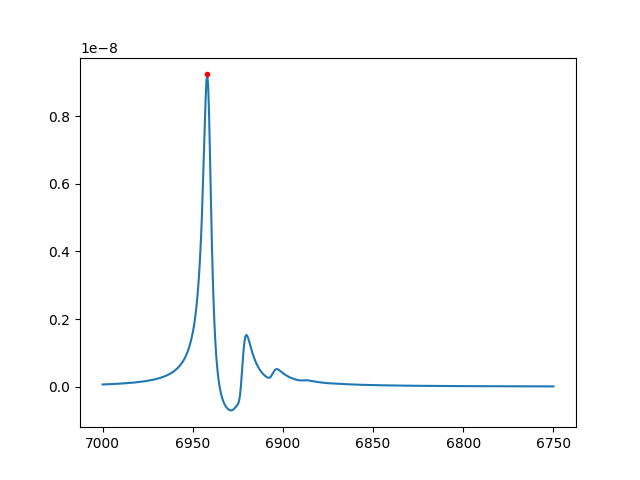
\includegraphics[width=0.9\linewidth]{erf=0.1,point6942.png}}
    \only<2>{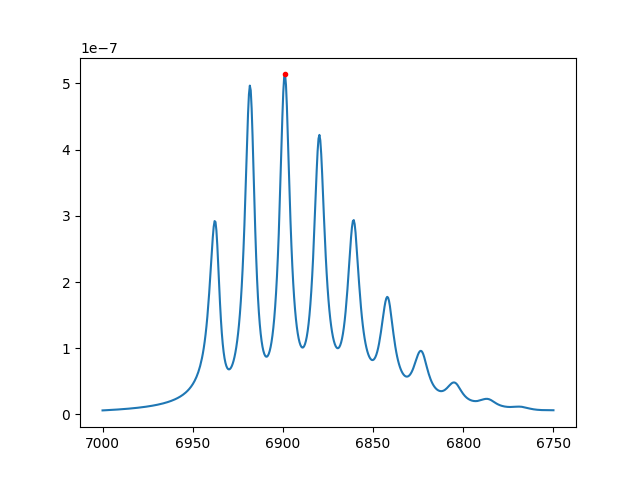
\includegraphics[width=0.9\linewidth]{erf=20,point6898.8.png}}
\end{column}%
\begin{column}{0.5\linewidth}
	\centering
    \only<1>{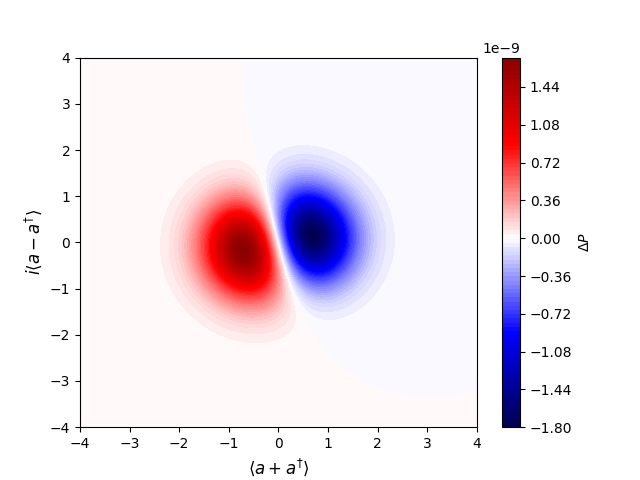
\includegraphics[width=0.9\linewidth]{erf=0.1,point6942,wignar.png}}
    \only<2>{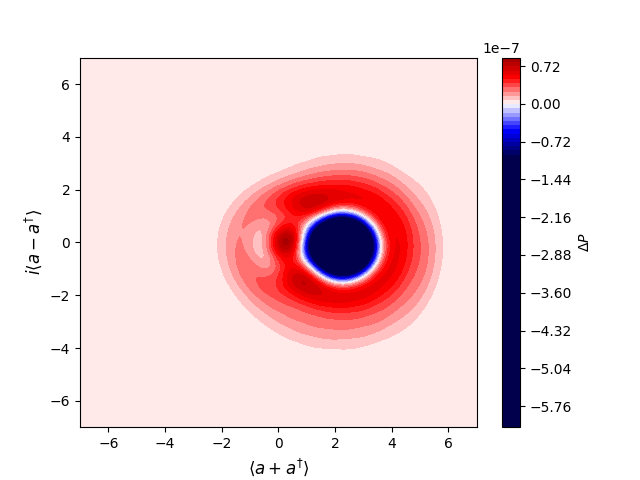
\includegraphics[width=0.9\linewidth]{erf=20,point6898.8,wignar.png}}
\end{column}
\end{columns}
\end{frame}

\section{Conclusion}
\begin{frame}[t]\frametitle{Conclusion}
\begin{itemize}
	\item Existence of photons in the cavity shifts the qubit frequency, 
	which can be read out by applying the sweeping signal to see the qubit 
	spectrum
	\item The way the qubit state affects the cavity state is trick: more 
	like polarization of qubit affect the wave function\pause
	\vspace{10pt}
	\item ``Approximately'' the peak hight can be interpreted as the photon 
	number distribution: ``Resolving'' photon number
	\item Potential application of quantum nondemolition measurement (QND)
\end{itemize}
\end{frame}

\begin{frame}%[allowframebreaks]
    \frametitle{Reference}
	\small
    % \printbibliography[heading=none]
    \bibliography{photonnumber}
\end{frame}

\begin{frame}\frametitle{The End...}
\centering
\Large
Thank you for listening! 
~\\
~\\

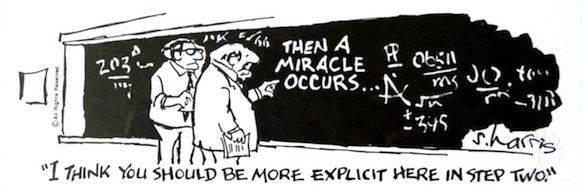
\includegraphics[width=0.9\linewidth]{miracle-occurs2.jpg}

Q \& A
\end{frame}

\appendix
% \section*{Circuit cQED}

% \begin{frame}
% \frametitle{Circuit Cavity QED}

% \only<1>{
% \begin{columns}
% \column{0.5\linewidth}
% \centering
% \begin{beamercolorbox}[wd={3cm}, ht={0.3cm},center, rounded=true,shadow=false]{postit}
% \textcolor{White}{Cavity}
% \end{beamercolorbox}
% \vspace{0.5cm}
% \begin{itemize}
% \item 1D transmission line resonator 
% \vspace{0.3cm}
% \item Full-wave section of superconducting coplanar waveguides
% \end{itemize}
% \vspace{0.3cm}
% \column{0.5\linewidth}
% \centering
% \begin{beamercolorbox}[wd={3cm}, ht={0.3cm},center, rounded=true,shadow=false]{postit}
% \textcolor{White}{Qubit}
% \end{beamercolorbox}
% \vspace{0.5cm}
% \begin{itemize}
% \item Cooper pair box
% \vspace{0.3cm}
% \item Superconducting mesoscopic island connected via a Josephson Junction to a reservoir
% \end{itemize}
% \end{columns}
% }
% \only<2>{
% \begin{figure}
% 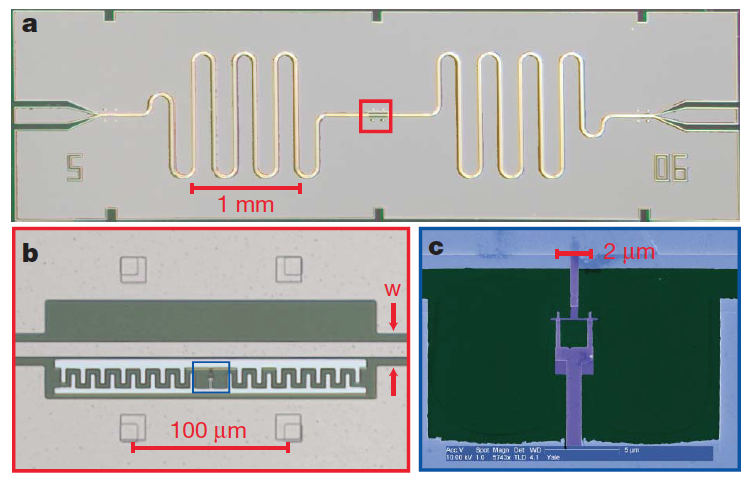
\includegraphics[width=0.8\linewidth]{Circuit}
% \caption{Cooper pair box inside a cavity, and spectral features of the
% circuit QED system.}
% \end{figure}
% \begin{center}
% \tiny{\textcolor{gray}{Image from Schuster, D. I., et al. "Resolving photon number states in a superconducting circuit." Nature 445.7127 (2007): 515-518.}}
% \end{center}}
% \end{frame}

\begin{frame}[t]\frametitle{Josephson junction and superconducting circuit}
% \begin{itemize}
	% \item Josephson junction $I = I_c\sin\phi$ with 
% \end{itemize}
\begin{columns}
	\begin{column}{0.75\linewidth}
	\begin{itemize}
		\item The Hamiltonian
		$$
			H = E_c (N-N_g)^2 - E_J\cos\delta
		$$
		\item Commutation relationship: $[\delta, N] = \mi$, this means 
		$\e^{\pm\mi\delta}\ket{n} = \ket{n\pm 1}$
	\end{itemize}
	\end{column}%
	\begin{column}{0.25\linewidth}
	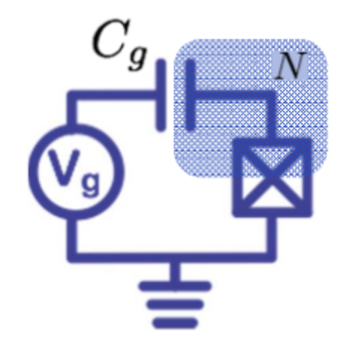
\includegraphics[width=\linewidth]{copper_pair_box.pdf}
	\end{column}
\end{columns}
\begin{itemize}
	\item Approximately two-level system: $0\le N_g \le 1$, $N = 0, 1$: 
	$$
	H = -E_c(1-2N_g) \sigma^z - \frac 12 E_J\sigma^x
	$$
	\item With coupling, $N_g \longrightarrow N_g + CV_0 (a + a^\dag)/2e$
	\item Choose eigen basis at degeneracy point ($N_g = 1/2$), we can have JC 
	model up to some constants. 
\end{itemize}
\end{frame}

\begin{frame}[t]\frametitle{Energy levels}
\begin{center}
	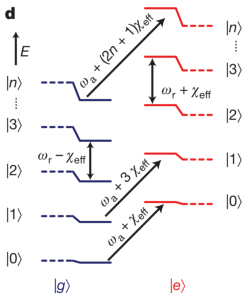
\includegraphics[height=0.85\textheight]{energy_levels.pdf}
\end{center}
\tiny{\textcolor{gray}{Image from Schuster, D. I., et al. "Resolving photon number states in a superconducting circuit." Nature 445.7127 (2007): 515-518.\cite{schuster2007resolving}}}
\end{frame}

\begin{frame}[t]\frametitle{Measurement}
In the experiment, the transmitted amplitude at frequency $\omega_{\rf}$ is the 
main observable. The exact way to measure can be found in Schuster's thesis \cite{schuster2007circuit}: 
\begin{center}
  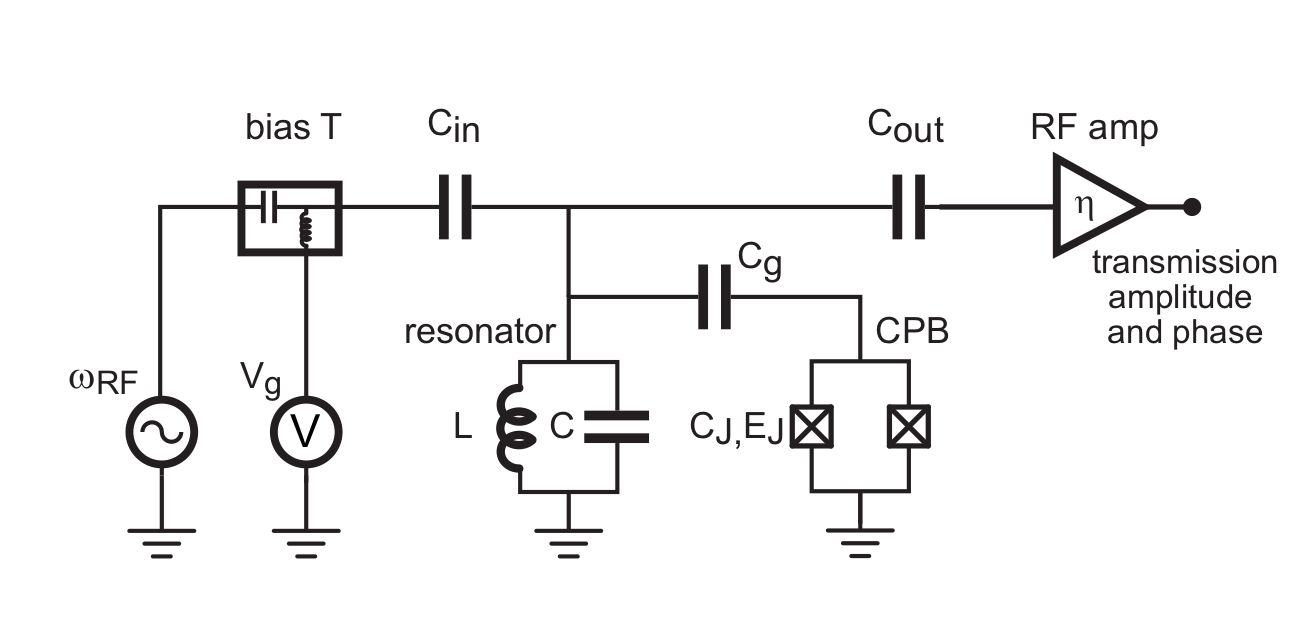
\includegraphics[width=0.6\textwidth]{measurement.png}
\end{center}
	\begin{itemize}
		\item What we really measure is the expectation of the voltage, or 
		electrical field $E\propto\langle a + a^\dag \rangle$
	\end{itemize}
\end{frame}

\begin{frame}[t]\frametitle{Wigner function (Wigner quasiprobability distribution)}
\begin{itemize}
	\item Wigner function is an analogue of classical probability distribution 
	on phase space
	\begin{block}{Definition: Wigner function}
	\begin{align*}
		P(x, p) &\equiv \frac{1}{(2\pi\hbar)^n}\int\dif^n y \,
		    \psi(x-y/2)\psi^*(x+y/2) \e^{\mi p\cdot y/\hbar} \\
		&= \frac{1}{(2\pi\hbar)^n}\int\dif^n y\, 
			\braket{x-y/2|\rho|x+y/2} \e^{\mi p\cdot y/\hbar}
	\end{align*}
	\end{block}
	\item Marginals: 
	\begin{align*}
		&\int\dif^n p\, P(x,p) = \braket{x|\rho|x} 
		&\int\dif^n x\, P(x,p) = \braket{p|\rho|p}
	\end{align*}
\end{itemize}
\end{frame}

\begin{frame}[t]\frametitle{Wigner function: properties}
\begin{itemize}
	\item Inner product $\rightarrow$ overlap: 
	$$
	  \left|\braket{\psi|\varphi}\right|^2 = 2\pi\hbar \int\dif^n x\dif^n p \,
	  P_\psi(x,p) P_\varphi(x,p)
	$$
	\item Operator Wigner transformation and expectation values: 
	\begin{align*}
		&g(x,p) \equiv \int\dif^n y \, \braket{x-y/2|G|x+y/2}
		\e^{\mi p\cdot y/\hbar} \\
		&\Tr [\rho G] = \int\dif^n x\dif^n p\, P(x,p)g(x,p)
	\end{align*}
	\item Cauchy inequality for pure state
	$$
	 -\frac 2h \le P(x,p) \le \frac 2h
	$$
\end{itemize}
\end{frame}


\end{document}
